%!TEX program = xelatex
% Note: this template must be compiled with XeLaTeX rather than PDFLaTeX
% due to the custom fonts used.
% Figures: scripts/pp/.venv/bin/python make_figures.py

\documentclass[
  aspectratio=169,
  t,
  onlytextwidth,
  10pt,
]{beamer}

\usepackage{../../ImperialTheme/beamer/beamerthemeImperial}
\usepackage{xcolor}
\usepackage{amsmath}
\usepackage{multirow}
\usepackage{booktabs}

\def\imagefolder{../../ImperialTheme/beamer/Images}
\def\Rey{\text{Re}}
\newcommand{\dd}{\mathrm{d}}
\newcommand{\awave}{\alpha}
\newcommand{\bU}{\boldsymbol{U}}
\newcommand{\bq}{\tilde{\boldsymbol{q}}}

\title{Local secondary (Floquet) stability of the 2D limit cycle in 3d domains at $d=1.5$}

\author{Víctor Ballester and Claude}

\date{9 November 2026}

\begin{document}

\begingroup
\setbeamercolor{background canvas}{bg=ICLLightGrey}
\setbeamercolor{title page title}{fg=ICLBlue}
\setbeamercolor{title page subtitle}{fg=ICLBlue}
\setbeamercolor{author}{fg=ICLBlue}
\setbeamercolor{date}{fg=ICLBlue}
\setbeamertemplate{title page}[logo]{\imagefolder/ICL_Logo_Blue.pdf}
\frame[plain, s]{\titlepage}
\endgroup

%----------------------------------------------------------------------
\begin{frame}
	\frametitle{Intro}
	\begin{itemize}
		\item $d=1.5$, $\Rey=1000$: widths $60 \leq w\leq 70$ have a 2D limit cycle (frequency similar to those convectivy unstable in BL).
		\item upstream noise amplitude changes the 3d breakdown point. So I (try to) ran Herbert local secondary analysis around the actual limit cycle.
		\end{itemize}
\end{frame}

%----------------------------------------------------------------------
\begin{frame}
	\frametitle{Base flow: locally parallel, but periodic}
	\begin{itemize}
		\item In the frame of the wave, $\xi=x-ct$, $c=\omega/\awave$, the 2D wave is steady. At a station $x_0$:
		      \[
			      \bU(\xi,y)=\underbrace{U_{BF}(y)+u_0(y)-c}_{n=0:\ \text{base + baseflow distortion}}\;+\sum_{n\neq0,\,|n|\leq3}\bU_n(y)\,e^{\mathrm{i}n\awave\xi}
		      \]
		\item we take $\omega$ from global LSA. $\alpha$ local approximation of the derivative (slowly varying in $x$), and the harmonics from least squares fitting in a neighbourhood of the point.
		\item The usual parallel-flow assumption (Orr--Sommerfeld) is the special case with no wave. Without the harmonics there is no secondary instability: the problem decouples into OS/Squire for each harmonic.
	\end{itemize}
\end{frame}

%----------------------------------------------------------------------
\begin{frame}
	\frametitle{Floquet problem}
	\begin{itemize}
		\item Base flow periodic in $\xi$ $\Rightarrow$ Floquet ansatz, normal modes in $z$ and $t$:
		      \[
			      \boldsymbol{q}'=\left(\sum_{m=-M}^{M}\bq_m(y)\,e^{\mathrm{i}m\awave\xi}\right)e^{\mathrm{i}\gamma\awave\xi}\,e^{\mathrm{i}\beta z}\,e^{\lambda t},
			      \qquad \gamma=0 \text{ (fundamental, K-type)},\ \tfrac12 \text{ (subharmonic, H-type)}
		      \]
		\item Each disturbance harmonic $m$, with $k_m=(m+\gamma)\awave$:
		      \[
			      \lambda\tilde{\boldsymbol{u}}_m=\tfrac{1}{\Rey}(\mathrm{D}^2-k_m^2-\beta^2)\tilde{\boldsymbol{u}}_m-\nabla_m\tilde p_m
			      -\sum_{n}\Big[(\mathrm{i}k_{m-n}U_{x,n}+U_{y,n}\mathrm{D})\tilde{\boldsymbol{u}}_{m-n}
				      +(\mathrm{i}n\awave\tilde u_{x,m-n}+\tilde u_{y,m-n}\mathrm{D})\bU_n\Big]
		      \]
		      Wave harmonic $n$ couples $m\leftrightarrow m-n$: this coupling is the instability.
		\item Temporal problem: $\beta$, $\gamma$ real, $\lambda$ complex eigenvalue: $\lambda\mathcal{M}\mathsf{q}=\mathcal{L}(\beta,\gamma)\mathsf{q}$.
		\item Numerics: Chebyshev collocation, 49 points, $y_{\max}=40$ (half below $y=2.5$), $N=M=3$ $\Rightarrow$ $1372\times1372$ matrix.
		      % \begin{itemize}
		      %  \item Validation: $N=0$ gives the Blasius critical point. 65 points, $M=5$, $y_{\max}=60$ changes $\sigma_t$ by $<0.5\%$.
		      % \end{itemize}
	\end{itemize}
\end{frame}

%----------------------------------------------------------------------
\begin{frame}
	\frametitle{From temporal to spatial growth}
	\begin{itemize}
		\item The eigenvalue problem gives a temporal growth: the 3D disturbance grows like $e^{\sigma_t t}$, $\sigma_t=\Re\lambda$.
		% \item The leading mode has $\lambda$ real ($|\Im\lambda|/\Re\lambda<10^{-9}$): it is locked to the wave, so it travels with it at speed $c$.
		\item After a time $t$ it has moved $x=ct$, so
		      \[
			      e^{\sigma_t t}=e^{(\sigma_t/c)\,x}
			      \quad\Longrightarrow\quad
			      \sigma=\frac{\sigma_t}{c}\quad\text{(spatial growth rate, Gaster)}
		      \]
	      \item In the DNS: we compute $\ln\|\zeta\|$ ($\zeta$ spanwise velocity, time and spanwise averaged, $L^2$ in $y$)
		\item $\beta$: the DNS box ($L_z=6$) only has $\beta_k=2\pi k/6$, so LSA $\sigma$ = max over those. The most amplified $\beta\approx0.5$--$0.67$ does not fit (i am running at larger box, twice as large now)
	\end{itemize}
\end{frame}

%----------------------------------------------------------------------
\begin{frame}
	\frametitle{Most unstable mode: $\sigma$ vs $\beta$ and $\gamma$}
	\begin{center}
		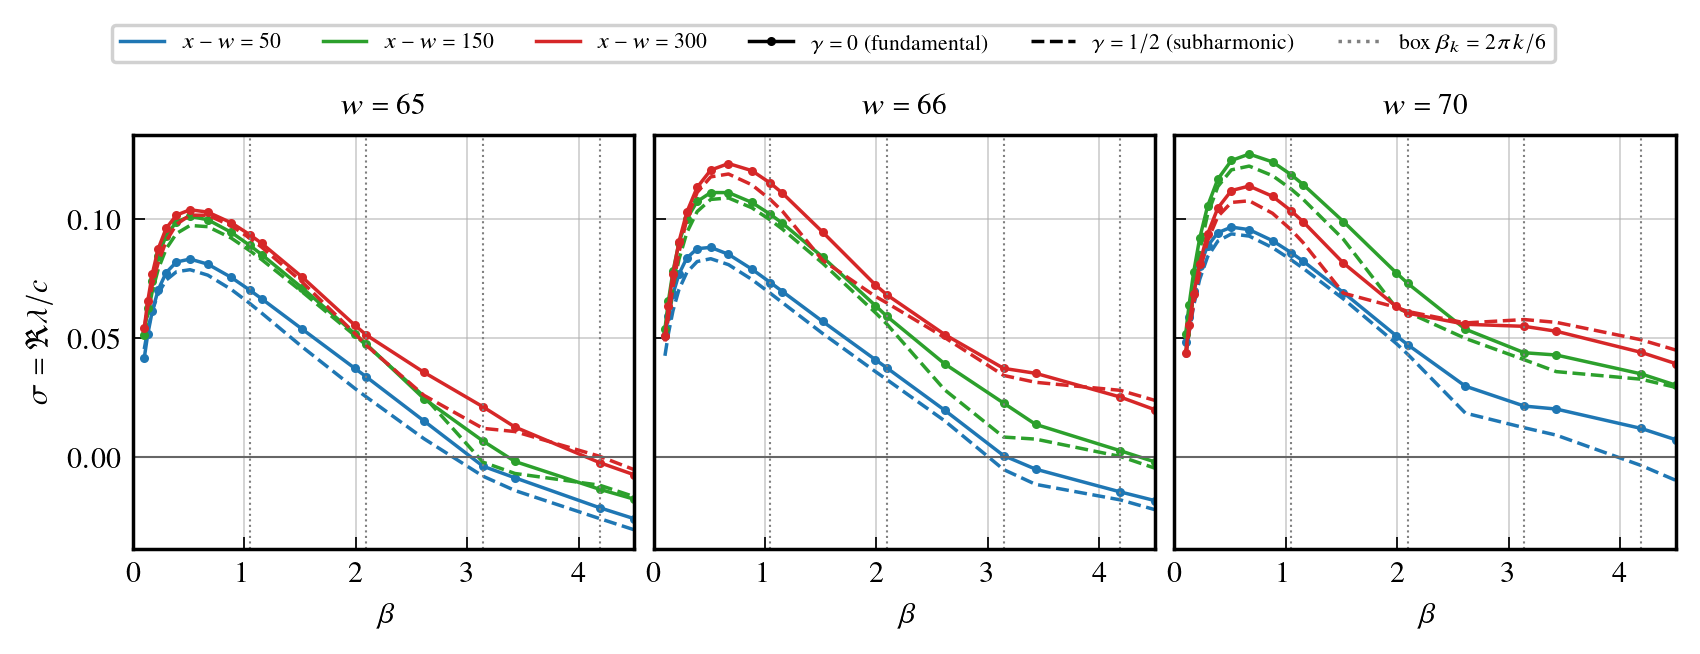
\includegraphics[width=0.8\linewidth]{Images/beta.png}
	\end{center}
	\vspace{-0.45cm}
	\small
	\begin{itemize}
		\item we compute $\gamma=0$ (fundamental, K-type) and $\gamma=1/2$ (subharmonic, H-type), 19 values of $\beta$.
		% \item at the peak the fundamental is slightly above (by $2$--$6\%$), so we use $\gamma=0$. Both are nearly equal, as expected for large-amplitude waves (Herbert 1988).
		% \item most unstable $\beta\approx0.5$ near the gap, $0.67$ downstream for $w=66,70$. In the box the best is $\beta_1=2\pi/6\approx1.05$: $8$--$15\%$ lower.
	\end{itemize}
\end{frame}

%----------------------------------------------------------------------
\begin{frame}
	\frametitle{Growth rates: LSA vs DNS}
	\begin{center}
		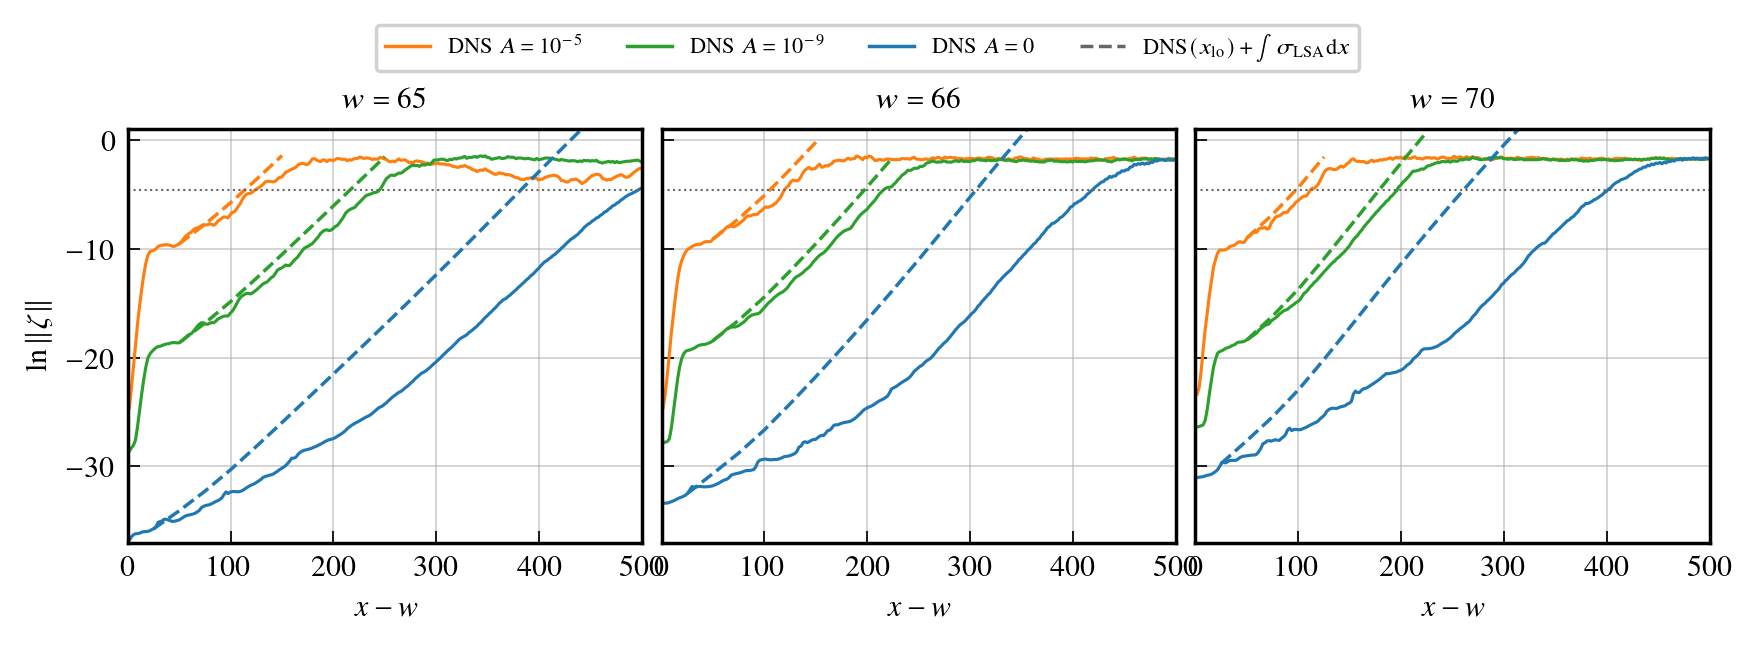
\includegraphics[width=\linewidth]{Images/dns.png}
	\end{center}
	\vspace{-0.3cm}
	\begin{itemize}
		\item solid: DNS $\ln\|\zeta\|$. Dashed: DNS$(x_{lo})+\int\sigma_{LSA}\dd x$, started where the linear stretch starts.
	\end{itemize}
\end{frame}

%----------------------------------------------------------------------
\begin{frame}
	\frametitle{Growth rates: numbers}
	\begin{columns}[T]
		\begin{column}{0.52\linewidth}
			\centering\footnotesize
			\renewcommand{\arraystretch}{0.95}
			\begin{tabular}{llccc}
				\toprule
				     &       & LSA (box) & \multicolumn{2}{c}{DNS} \\
				\cmidrule(lr){4-5}
				$w$  & $x-w$ &           & $A=10^{-9}$ & $A=0$ \\
				\midrule
				\multirow{4}{*}{65} & 100 & 0.084 & 0.074 & 0.042 \\
				                    & 150 & 0.089 & 0.078 & 0.064 \\
				                    & 200 & 0.090 & 0.079 & 0.053 \\
				                    & 300 & 0.093 & --    & 0.084 \\
				\midrule
				\multirow{4}{*}{66} & 100 & 0.094 & 0.074 & 0.035 \\
				                    & 150 & 0.102 & 0.093 & 0.059 \\
				                    & 200 & 0.108 & --    & 0.063 \\
				                    & 300 & 0.115 & --    & 0.104 \\
				\midrule
				\multirow{4}{*}{70} & 100 & 0.109 & 0.088 & 0.042 \\
				                    & 150 & 0.118 & 0.109 & 0.061 \\
				                    & 200 & 0.116 & --    & 0.061 \\
				                    & 300 & 0.103 & --    & 0.099 \\
				\bottomrule
			\end{tabular}
		\end{column}
		\begin{column}{0.46\linewidth}
			\small
			Mean ratio $\sigma_{DNS}/\sigma_{LSA}$:
			\vspace{0.1cm}

			\renewcommand{\arraystretch}{1.1}
			\begin{tabular}{lcc}
				\toprule
				         & $x-w\geq100$ & $x-w\geq250$ \\
				\midrule
				$A=10^{-9}$ & 0.87--0.88 & --  \\
				$A=0$       & 0.65--0.77 & 0.88--0.89 \\
				\bottomrule
			\end{tabular}
			\begin{itemize}
				\item ranges over $w=65,66,70$.
				\item --: already saturated ($\|\zeta\|>10^{-2.5}$).
			\end{itemize}
		\end{column}
	\end{columns}
\end{frame}


\end{document}
